
\documentclass[conference]{IEEEtran}
\usepackage{blindtext, graphicx}
\usepackage{multirow}
\usepackage{float}
\usepackage{amsmath}
\usepackage[section]{placeins}
\usepackage{amsthm}
\usepackage{eucal}
\usepackage{amssymb}
\usepackage{mathrsfs}
\usepackage{pgfplotstable}
\usepackage{pgfplots}
\hyphenation{op-tical net-works semi-conduc-tor}

\begin{document}
\title{Performance Analysis of Parallel Collaborative Filtering on Spark and Hadoop cluster}

\author{\IEEEauthorblockN{Kundjanasith Thonglek}
\IEEEauthorblockA{High Performance Computing and Network Center\\
Deparment of Computer Engineering, Kasetsart University\\
Bangkok, Thailand\\
kundjanasith.t@ku.th}
\and
\IEEEauthorblockN{Kohei Ichikawa}
\IEEEauthorblockA{Software Design and Analysis Laboratory\\
Graduate School of Information Science, NAIST\\
Nara, Japan\\
ichikawa@is.naist.jp}}
%\and
%\IEEEauthorblockN{James Kirk\\ and Montgomery Scott}
%\IEEEauthorblockA{Starfleet Academy\\
%San Francisco, California 96678-2391\\
%Telephone: (800) 555--1212\\
%Fax: (888) 555--1212}}
\maketitle


\begin{abstract}
Spark is a cluster computing technology for large-scale data processing that provides an interface for programming entire clusters with implicit data parallelism and fault tolerance. Following the SparkContext can connect to several types of cluster manager which allocate resource across applications. Once connected, Spark acquires executors on nodes in the cluster, which are processes that run computations and store data for the application. Next, it sends application code to the executors. SparkContext represents the connection to a Spark cluster and can be used to create resilient distributed datasets (RDDs). it also accumulators and broadcast variables on the cluster. This research approaches the problem by comparing Spark cluster and Hadoop cluster performance are used the parallel collaborative filtering program?s execution time as criteria to find when the application should execute on Spark or Hadoop. This research is primarily intended for cluster computing benchmark.
\end{abstract}

\begin{IEEEkeywords}
Large scale data processing; Resilient Distributed Datasets; Collaborative Filtering; Spark;
\end{IEEEkeywords}


\section{Introduction}
Big data and advanced analytics technology is not just because the size of data is big but also because the potential of impact is big such as recommendation system, clustering system and the others. They were not possible previously because they were too costly to implement or they were not capable of handling the large volumes of data involved in a timely manner. But in the present technology can make it possible due to the new data management systems that handle a wide variety of data from sensor data to web and social media data improved analytical capabilities including event, predictive and text analytics, faster hardware ranging from faster multi-core processors and large memory space to solid-state drives and tried data storage for handling data. Supporting big data involves combining these technologies to enable new solutions that can bring significant benefits to the business.\\
\indent Recommendation system is the key to success for discovering and retrieval of content in this era of big data. It have become increasingly popular in recent years, and are utilized in a variety of areas including movies, music, news, books, and product in general. These are also recommendation for experts. Collaborative Filtering (CF) technique is used to create recommendation system, is a technique of making automatic predictions about interest of a user by collecting preference or taste information from many users. The advantages of this technique are not rely on machine analyzable content, it is capable of accurately recommending complex items such as movies movies without requiring an understanding of the item similarity in recommendation system. The technique is based on the assumption that people who agreed in the past will agree in the future, and they will like similar kinds of items as they liked in the past. The algorithm is widely applied to this technique is Alternating Least Square (ALS) algorithm that aim at learning the two types of items as they liked in the past.\\
\indent Large-scale data processing is the process of applying data analysis technique to a large amount of data. Typically, large-scale data analysis is performed through two popular techniques: parallel database management systems or map reduce powers systems. The parallel database management system requires that the data be in a database management system supported schema, whereas map reduce system supports data in any form. Moreover, the dat extracted or analyzed in large-scale data analysis can be displayed in various different forms such as tables, graphs, figures and statistical analysis that depending on the analysis system. There are two popular open source cluster computing for large-scale data processing based on the map reduce model: Spark framework which is the framework process data by in-memory processing, has Spark ML library to be scalable machine learning library and Hadoop framework which is the framework process data by on-disk processing, has Mahout library to be scalable machine learning library.

%\subsection{Subsection Heading Here}
%\blindtext

\section{Literature review}
\subsection{Large-scale Parallel Collaborative Filtering for Netflix}
Spark ML library and Mahout library are scalable machine learning library use this paper to be the reference for parallel collaborative filtering technique using alternating least square algorithm to implement in the library of both. However, this paper execute the parallel collaborative filtering technique using Matlab library on Linux cluster only. \\
\indent This research will further advance paper by executing parallel collaborative filtering technique using more efficient framework than using Matlab library on Linux cluster with Spark ML library on Spark cluster and Mahout library on Hadoop cluster. 

\subsection{Comparing Apache Spark and MapReduce with Performance Analysis using K-Means}
K-means clustering algorithm is the algorithm that simpler than Alternating Least Square algorithm is used to apply with parallel collaborative filtering technique. Spark and Hadoop cluster with 1 node and 2 nodes is too small to find the impact of the number of node on the executing performance. \\
\indent This research will further advance paper by using the alternating least square algorithm of parallel collaborative technique instead of K-means algorithm because of the complexity. The environment of experimental cluster is extended to 5 worker nodes that can find the impact or relation to the performance with increasing the number of worker nodes. 

\section{Design and Implementation}
There are 2 large-scale data processing framework which we use in the experiment are Spark framework and Hadoop framework. Spark using in-memory processing to process data but Hadoop using on-disk processing. \\
\indent  Alternating Least Square (ALS) algorithm is CPU intensive algorithm more than memory intensive so we design experiment by vary the number of CPU cores per each worker node with fix the size of memory per each worker node. We interest the number of worker nodes effect to the performance or not then we design the experiment by changing the number of worker nodes in the cluster with the same total number of CPU cores and memory size in the cluster. \\
\indent We find the dataset that suitable to create recommendation system by parallel collaborative filtering technique is dataset from The Netflix Prize that is a large-scale data mining competition held by Netflix for the best recommendation system algorithm for predicting user ratings on movies, based on a training set of more than 100 million ratings given by over 480,000 users to nearly 18,000 movies. Each training data point consist of a quadruple ( user, movie, date, rating ) where the rating is an integer from 1 to 5, the size of dataset is 2.8 gb. Afterward, we separate the dataset using sampling to 20 datasets by starting from 5 million records then add up 5 million util 100 million records. \\
\indent Experiment is divided into 2 sections to find the suitable configuration of Spark cluster and Hadoop cluster in the limited resource to executer parallel collaborative filtering technique for create the recommendation system: First section is the number of CPU cores per each worker node effect analysis to observe parallel computing by changing the number of CPU cores per each worker node to 2, 4, 8, 16 with fix the size of memory is 8 gb per each worker node and Second section is the number of worker node effect analysis to observer parallel I/O by changing the number of worker node with the total number of CPU cores is 20 and size of memory is  40 gb. \\
\indent Implementation is divided into three main parts in this experiment. The first part is installation part, the second part is training data part, the third part is performance analysis part. Installation part is a  part for installation and configuration the Spark and Hadoop on cluster. Training data part is a part for training data  for train data by Spark ML library on the Spark cluster and Mahout library on Hadoop cluster.  Performance analysis part is a part for analyst the execution time of each configuration. 

\subsection{Installation Part}
Installation Part has 2 sections: First section is the installation part for observe parallel computing effect and second section is the installation part for observe parallel I/O effect. \\
\indent The configuration in cluster of parallel computing observation:
\begin{itemize}
\item Case 1 : 5 worker nodes by each node has CPU 2 cores and memory 8 gb
\item Case 2 : 5 worker nodes by each node has CPU 4 cores and memory 8 gb
\item Case 3 : 5 worker nodes by each node has CPU 8 cores and memory 8 gb
\item Case 4 : 5 worker nodes by each node has CPU 16 cores and memory 8 gb
\end{itemize}
\indent The configuration in cluster of parallel I/O observation:
\begin{itemize}
\item Case 1 : 5 worker nodes by each node has CPU 4 cores and memory 8 gb
\item Case 2 : 4 worker nodes by each node has CPU 5 cores and memory 10 gb
\item Case 3 : 2 worker nodes by each node has CPU 10 cores and memory 20 gb
\item Case 4 : 1 worker node which has CPU 20 cores and memory 40 gb
\end{itemize}

\subsection{Training data Part}
Training data Part has 2 sections: Using Spark ML library on Spark cluster and Mahout library on Hadoop cluster which have the same alternating least square algorithm implementation on both libraries. \\
\indent The Parallel Alternating-Least-Squares with Weighted-\begin{math}\lambda\end{math}-Regularization (ALS-WR) algorithm  is parallelized by parallelizing the updates of the user feature matrix and of the movie feature matrix.


\subsection{Performance analysis Part}
Performance analysis Part has 3 sections: Recording time information using time command,  Calculate the average value of time in second unit due to we give a trial three times per each condition and evaluate the result from the experiment by R programming language.\\
\indent For the number of CPU cores per each worker node effect analysis to observer parallel computing. There are 2 dependent variables on time variable: the number of CPU cores per each worker node and the size of dataset.\\
\indent Let \textbf{\textit{t}} be the execution time (seconds)\\
\indent Let \textbf{\textit{c}} be the number of CPU core per worker node (cores)\\
\indent Let \textbf{\textit{d}} be the size of data set (MB)\\
\indent The Multiple linear regression (MLR) model that describes a dependent variable  \textbf{\textit{t}} by independent variables \textbf{\textit{c}} and  \textbf{\textit{d}} is expressed by the equation as follow where the number \begin{math}\alpha\end{math} and \begin{math}\beta\end{math} are the parameters, and \begin{math}\phi\end{math} is the error term (1).

\indent For the number of worker nodes effect analysis to observer parallel I/O. There are 2 dependent variables on time variable: the number of worker nodes and the size of dataset.\\
\indent Let \textbf{\textit{t}} be the execution time (seconds)\\
\indent Let \textbf{\textit{n}} be the number of worker node (nodes)\\
\indent Let \textbf{\textit{d}} be the size of data set (MB)\\
\indent The Multiple linear regression (MLR) model that describes a dependent variable  \textbf{\textit{t}} by independent variables \textbf{\textit{n}} and  \textbf{\textit{d}} is expressed by the equation as follow where the number \begin{math}\alpha\end{math} and \begin{math}\beta\end{math} are the parameters, and \begin{math}\phi\end{math} is the error term (2).

\begin{equation}
	t = \alpha + \beta_{1}c + \beta_{2}d + \phi
\end{equation}
\begin{equation}
	t = \alpha + \beta_{1}n + \beta_{2}d + \phi
\end{equation}

\section{Experiment result}
After we give a trial for execute the different size of data sets with the same algorithm but different type of cluster configuration. The experimental result is divided to 2 sections.\\
\indent First section is the experimental result of executing parallel collaborative filtering using alternating least square algorithm with Spark ML library on Spark cluster and Mahout library on Hadoop cluster by changing the number of CPU cores per worker node in the cluster which has 1 master node and 5 worker nodes for observe the impact from parallel computing on the performance. 

\begin{figure}[h]
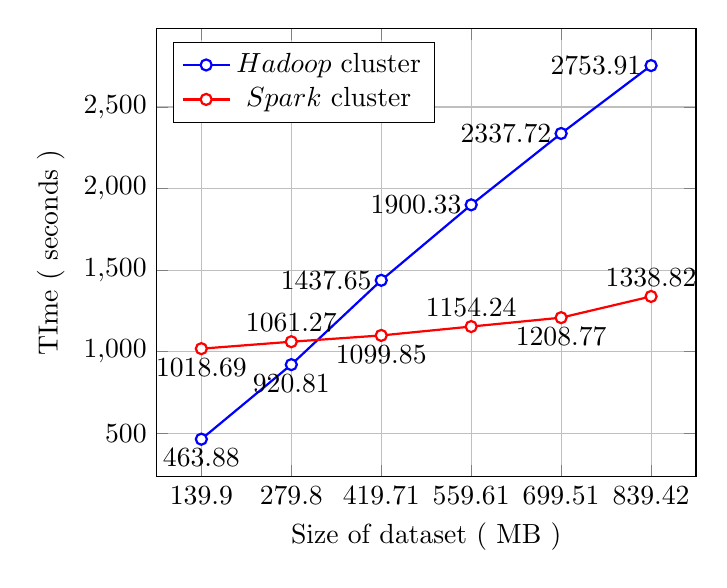
\begin{tikzpicture}
\begin{axis}[
	xlabel=Size of dataset ( MB ),
	ylabel=TIme ( seconds ), 
	xtick={139.90, 279.80, 419.71, 559.61, 699.51, 839.42},
	grid=both,
	legend pos=north west]
%\addplot table [y=$Hadoop$, x=Size]{latex_data/HS_C1.dat};
\addplot[color=blue,solid,thick,mark=*, mark options={fill=white}] 
    coordinates {
         (139.90, 463.88)
         (279.80, 920.81)
         (419.71, 1437.65)
         (559.61, 1900.33)
         (699.51, 2337.72)
         (839.42, 2753.91)
    }; 
\node [below] at (axis cs:  139.90, 463.88) {$463.88$};
\node [below] at (axis cs:  279.80, 920.81) {$920.81$};
\node [left] at (axis cs: 419.71, 1437.65) {$1437.65$};
\node [left] at (axis cs: 559.61, 1900.33) {$1900.33$};
\node [left] at (axis cs: 699.51, 2337.72) {$2337.72$};
\node [left] at (axis cs: 839.42, 2753.91) {$2753.91$};
\addlegendentry{$Hadoop$  cluster}
%\addplot table [y=$Spark$, x=Size]{latex_data/HS_C1.dat};
\addplot[color=red,solid,thick,mark=*, mark options={fill=white}] 
    coordinates {
         (139.90, 1018.69)
         (279.80, 1061.27)
         (419.71, 1099.85)
         (559.61, 1154.24)
         (699.51, 1208.77)
         (839.42, 1338.82)
    }; 
\node [below] at (axis cs:  139.90, 1018.69) {$1018.69$};
\node [above] at (axis cs:  279.80, 1061.27) {$1061.27$};
\node [below] at (axis cs: 419.71, 1099.85) {$1099.85$};
\node [above] at (axis cs: 559.61, 1154.24) {$1154.24$};
\node [below] at (axis cs: 699.51, 1208.77) {$1208.77$};
\node [above] at (axis cs: 839.42,1338.82) {$1338.82$};
\addlegendentry{$Spark$ cluster}
\end{axis}
\end{tikzpicture}
\caption{Graph of testing on 5 workers node by each node has CPU 2 cores and memory 8 GB}
\end{figure}
From Fig 1, we can analyze that the intersection point between Hadoop cluster line and Spark cluster line at the size of dataset is  319.51 MB and the execution time is 1074.05 seconds

\begin{figure}[H]
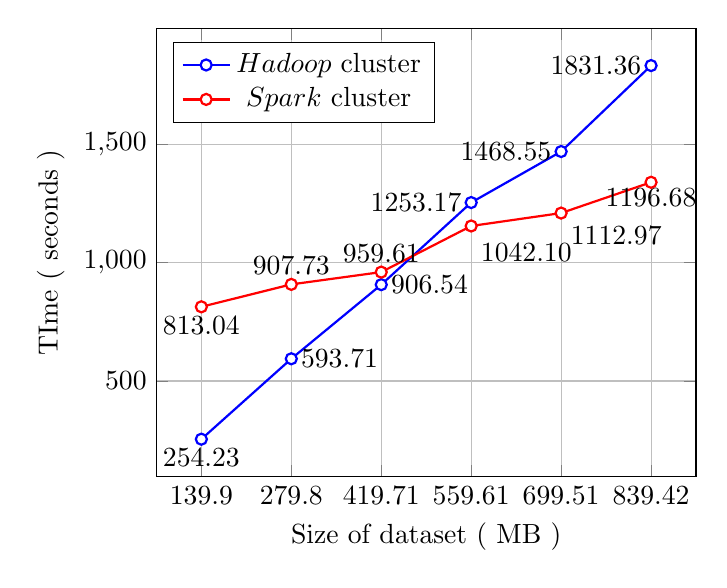
\begin{tikzpicture}
\begin{axis}[
	xlabel=Size of dataset ( MB ),
	ylabel=TIme ( seconds ),
	xtick={139.90, 279.80, 419.71, 559.61, 699.51, 839.42},
	grid=both, 
	legend pos=north west]
%\addplot table [y=$Hadoop$, x=Size]{latex_data/HS_C2.dat};
\addplot[color=blue,solid,thick,mark=*, mark options={fill=white}] 
    coordinates {
         (139.90, 254.23)
         (279.80, 593.71)
         (419.71, 906.54)
         (559.61, 1253.17)
         (699.51, 1468.55)
         (839.42, 1831.36)
    }; 
\node [below] at (axis cs:  139.90, 254.23) {$254.23$};
\node [right] at (axis cs:  279.80, 593.71) {$593.71$};
\node [right] at (axis cs: 419.71, 906.54) {$906.54$};
\node [left] at (axis cs: 559.61, 1253.17) {$1253.17$};
\node [left] at (axis cs: 699.51, 1468.55) {$1468.55$};
\node [left] at (axis cs: 839.42, 1831.36) {$1831.36$};
\addlegendentry{$Hadoop$  cluster}
%\addplot table [y=$Spark$, x=Size]{latex_data/HS_C2.dat};
\addplot[color=red,solid,thick,mark=*, mark options={fill=white}] 
    coordinates {
         (139.90, 813.04)
         (279.80, 907.73)
         (419.71, 959.61)
         (559.61, 1154.24)
         (699.51, 1208.77)
         (839.42, 1338.82)
    }; 
\node [below] at (axis cs:  139.90, 813.04) {$813.04$};
\node [above] at (axis cs:  279.80, 907.73) {$907.73$};
\node [above] at (axis cs: 419.71, 959.61) {$959.61$};
\node [right] at (axis cs: 559.61, 1042.10) {$1042.10$};
\node [right] at (axis cs: 699.51, 1112.97) {$1112.97$};
\node [above] at (axis cs: 839.42,1196.68) {$1196.68$};
\addlegendentry{$Spark$ cluster}
\end{axis}
\end{tikzpicture}
\caption{Graph of testing on 5 workers node by each node has CPU 4 cores and memory 8 GB}
\end{figure}
From Fig 2, we can analyze that the intersection point between Hadoop cluster line and Spark cluster line at the size of dataset is 462.38 MB and the execution time is 990.78 seconds

\begin{figure}[H]
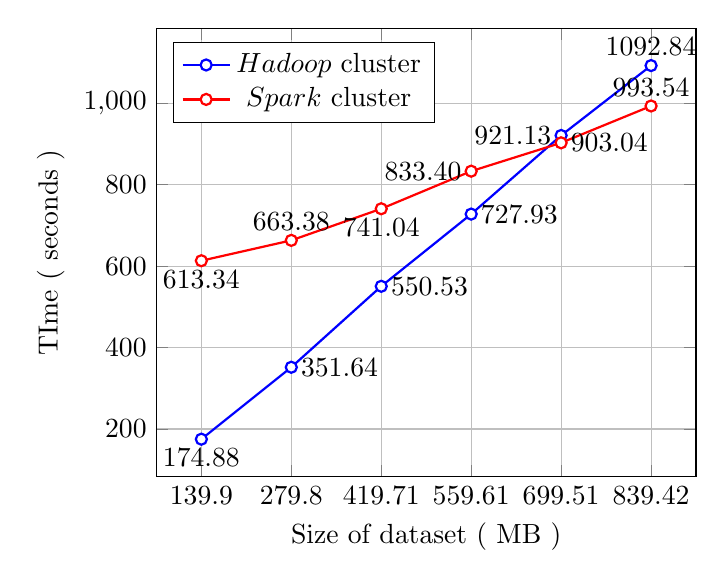
\begin{tikzpicture}
\begin{axis}[
	xlabel=Size of dataset ( MB ),
	ylabel=TIme ( seconds ), 
	xtick={139.90, 279.80, 419.71, 559.61, 699.51, 839.42},
	grid=both, 
	legend pos=north west]
%\addplot table [y=$Hadoop$, x=Size]{latex_data/HS_C3.dat};
\addplot[color=blue,solid,thick,mark=*, mark options={fill=white}] 
    coordinates {
         (139.90, 174.88)
         (279.80, 351.64)
         (419.71, 550.53)
         (559.61, 727.93)
         (699.51, 921.13)
         (839.42, 1092.84)
    }; 
\node [below] at (axis cs:  139.90, 174.88) {$174.88$};
\node [right] at (axis cs:  279.80, 351.64) {$351.64$};
\node [right] at (axis cs: 419.71, 550.53) {$550.53$};
\node [right] at (axis cs: 559.61, 727.93) {$727.93$};
\node [left] at (axis cs: 699.51, 921.13) {$921.13$};
\node [above] at (axis cs: 839.42, 1092.84) {$1092.84$};
\addlegendentry{$Hadoop$  cluster}
%\addplot table [y=$Spark$, x=Size]{latex_data/HS_C3.dat};
\addplot[color=red,solid,thick,mark=*, mark options={fill=white}] 
    coordinates {
         (139.90, 613.34)
         (279.80, 663.38)
         (419.71, 741.04)
         (559.61, 833.40)
         (699.51, 903.04)
         (839.42, 993.54)
    }; 
\node [below] at (axis cs:  139.90, 613.34) {$613.34$};
\node [above] at (axis cs:  279.80, 663.38) {$663.38$};
\node [below] at (axis cs: 419.71, 741.04) {$741.04$};
\node [left] at (axis cs: 559.61, 833.40) {$833.40$};
\node [right] at (axis cs: 699.51, 903.04) {$903.04$};
\node [above] at (axis cs: 839.42, 993.54) {$993.54$};
\addlegendentry{$Spark$ cluster}
\end{axis}
\end{tikzpicture}
\caption{Graph of testing on 5 workers node by each node has CPU 8 cores and memory 8 GB}
\end{figure}
From Fig 3, we can analyze that the intersection point between Hadoop cluster line and Spark cluster line at the size of dataset is 691.07 MB and the execution time is 902.86 seconds

\begin{figure}[H]
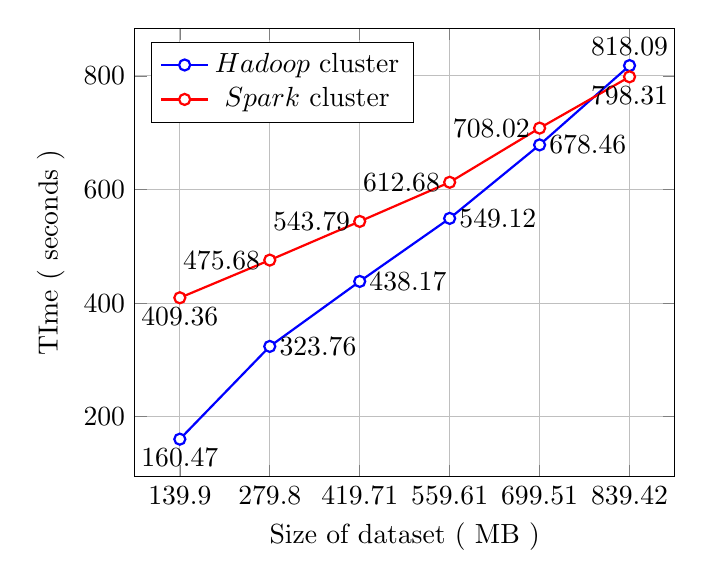
\begin{tikzpicture}
\begin{axis}[
	xlabel=Size of dataset ( MB ),
	ylabel=TIme ( seconds ), 
	xtick={139.90, 279.80, 419.71, 559.61, 699.51, 839.42},
	grid=both, 
	legend pos=north west]
%\addplot table [y=$Hadoop$, x=Size]{latex_data/HS_C4.dat};
\addplot[color=blue,solid,thick,mark=*, mark options={fill=white}] 
    coordinates {
         (139.90, 160.47)
         (279.80, 323.76)
         (419.71, 438.17)
         (559.61, 549.12)
         (699.51, 678.46)
         (839.42, 818.09)
    }; 
\node [below] at (axis cs:  139.90, 160.47) {$160.47$};
\node [right] at (axis cs:  279.80, 323.76) {$323.76$};
\node [right] at (axis cs: 419.71, 438.17) {$438.17$};
\node [right] at (axis cs: 559.61, 549.12) {$549.12$};
\node [right] at (axis cs: 699.51, 678.46) {$678.46$};
\node [above] at (axis cs: 839.42, 818.09) {$818.09$};
\addlegendentry{$Hadoop$  cluster}
%\addplot table [y=$Spark$, x=Size]{latex_data/HS_C4.dat};
\addplot[color=red,solid,thick,mark=*, mark options={fill=white}] 
    coordinates {
         (139.90, 409.36)
         (279.80, 475.68)
         (419.71, 543.79)
         (559.61, 612.68)
         (699.51, 708.02)
         (839.42, 798.31)
    }; 
\node [below] at (axis cs:  139.90, 409.36) {$409.36$};
\node [left] at (axis cs:  279.80, 475.6) {$475.68$};
\node [left] at (axis cs: 419.71, 543.79) {$543.79$};
\node [left] at (axis cs: 559.61, 612.68) {$612.68$};
\node [left] at (axis cs: 699.51, 708.02) {$708.02$};
\node [below] at (axis cs: 839.42, 798.31) {$798.31$};
\addlegendentry{$Spark$ cluster}
\end{axis}
\end{tikzpicture}
\caption{Graph of testing on 5 workers node by each node has CPU 16 cores and memory 8 GB}
\end{figure}
From Fig 4, we can analyze that the intersection point between Hadoop cluster line and Spark cluster line at the size of dataset is 759.62 MB and the execution time is 740.75 seconds

\begin{table}[h]
\centering
\caption{The intersection point of each configuration that observe parallel computing }
\label{my-label}
\begin{tabular}{|c|c|c|}
\hline
\multirow{2}{*}{The configuration in cluster} & \multirow{2}{*}{\begin{tabular}[c]{@{}c@{}}Size of dataset\\ ( MB )\end{tabular}} & \multirow{2}{*}{\begin{tabular}[c]{@{}c@{}}Execution time\\ ( seconds )\end{tabular}} \\
 &  &  \\ \hline
\begin{tabular}[c]{@{}c@{}}5 worker nodes by each node \\ has CPU 2 cores and memory 8 gb\end{tabular} & 319.51 & 1074.05 \\ \hline
\begin{tabular}[c]{@{}c@{}}5 worker nodes by each node\\ has CPU 4 cores and memory 8 gb\end{tabular} & 462.38 & 990.78 \\ \hline
\begin{tabular}[c]{@{}c@{}}5 worker nodes by each node \\ has CPU 8 cores and memory 8 gb\end{tabular} & 691.07 & 902.86 \\ \hline
\begin{tabular}[c]{@{}c@{}}5 worker nodes by each node\\ has CPU 16 cores and memory 8 gb\end{tabular} & 759.62 & 740.75 \\ \hline
\end{tabular}
\end{table}
When we increase the number of CPU cores per each worker node in cluster,  the intersection point between Hadoop line and Spark line will cross at the higher size of dataset and the lower execution time 


\section{Conclusion}







% if have a single appendix:
%\appendix[Proof of the Zonklar Equations]
% or
%\appendix  % for no appendix heading
% do not use \section anymore after \appendix, only \section*
% is possibly needed

% use appendices with more than one appendix
% then use \section to start each appendix
% you must declare a \section before using any
% \subsection or using \label (\appendices by itself
% starts a section numbered zero.)
%


\appendices
\section{Proof of the First Zonklar Equation}
\blindtext

% use section* for acknowledgement
\section*{Acknowledgment}


The authors would like to thank...


% Can use something like this to put references on a page
% by themselves when using endfloat and the captionsoff option.
\ifCLASSOPTIONcaptionsoff
  \newpage
\fi



% trigger a \newpage just before the given reference
% number - used to balance the columns on the last page
% adjust value as needed - may need to be readjusted if
% the document is modified later
%\IEEEtriggeratref{8}
% The "triggered" command can be changed if desired:
%\IEEEtriggercmd{\enlargethispage{-5in}}

% references section

% can use a bibliography generated by BibTeX as a .bbl file
% BibTeX documentation can be easily obtained at:
% http://www.ctan.org/tex-archive/biblio/bibtex/contrib/doc/
% The IEEEtran BibTeX style support page is at:
% http://www.michaelshell.org/tex/ieeetran/bibtex/
%\bibliographystyle{IEEEtran}
% argument is your BibTeX string definitions and bibliography database(s)
%\bibliography{IEEEabrv,../bib/paper}
%
% <OR> manually copy in the resultant .bbl file
% set second argument of \begin to the number of references
% (used to reserve space for the reference number labels box)
\begin{thebibliography}{1}

\bibitem{IEEEhowto:kopka}
H.~Kopka and P.~W. Daly, \emph{A Guide to \LaTeX}, 3rd~ed.\hskip 1em plus
  0.5em minus 0.4em\relax Harlow, England: Addison-Wesley, 1999.

\end{thebibliography}

% biography section
% 
% If you have an EPS/PDF photo (graphicx package needed) extra braces are
% needed around the contents of the optional argument to biography to prevent
% the LaTeX parser from getting confused when it sees the complicated
% \includegraphics command within an optional argument. (You could create
% your own custom macro containing the \includegraphics command to make things
% simpler here.)
%\begin{biography}[{\includegraphics[width=1in,height=1.25in,clip,keepaspectratio]{mshell}}]{Michael Shell}
% or if you just want to reserve a space for a photo:

\begin{IEEEbiography}[{\includegraphics[width=1in,height=1.25in,clip,keepaspectratio]{picture}}]{John Doe}
\blindtext
\end{IEEEbiography}

% You can push biographies down or up by placing
% a \vfill before or after them. The appropriate
% use of \vfill depends on what kind of text is
% on the last page and whether or not the columns
% are being equalized.

%\vfill

% Can be used to pull up biographies so that the bottom of the last one
% is flush with the other column.
%\enlargethispage{-5in}




% that's all folks
\end{document}


